\documentclass{beamer}
\mode<presentation>
\usepackage{ICES_beamer_template}
\usepackage[english]{babel}
\usepackage[utf8x]{inputenc}
\usepackage{amsmath,bm}

%===============================================================================
% 					  Presentation Title and Author  
%===============================================================================
\title[Updates]{Updates: Data/Images for Fenics}
\author{Xoab Perez}
\date{\today}

\begin{document}

\begin{frame}
  \titlepage
\end{frame}

% Uncomment these lines for an automatically generated outline.
%\begin{frame}{Outline}
% \tableofcontents
%\end{frame}

%===============================================================================
% SLIDE 01
\section{Data for Fenics}
\subsection{Total Growth}
%===============================================================================

\begin{frame}{Comparisons of Tumor Growth Between Rats}
	\begin{minipage}[T][.7\textheight][t]{\textwidth}
		\begin{figure}
    	\centering
    	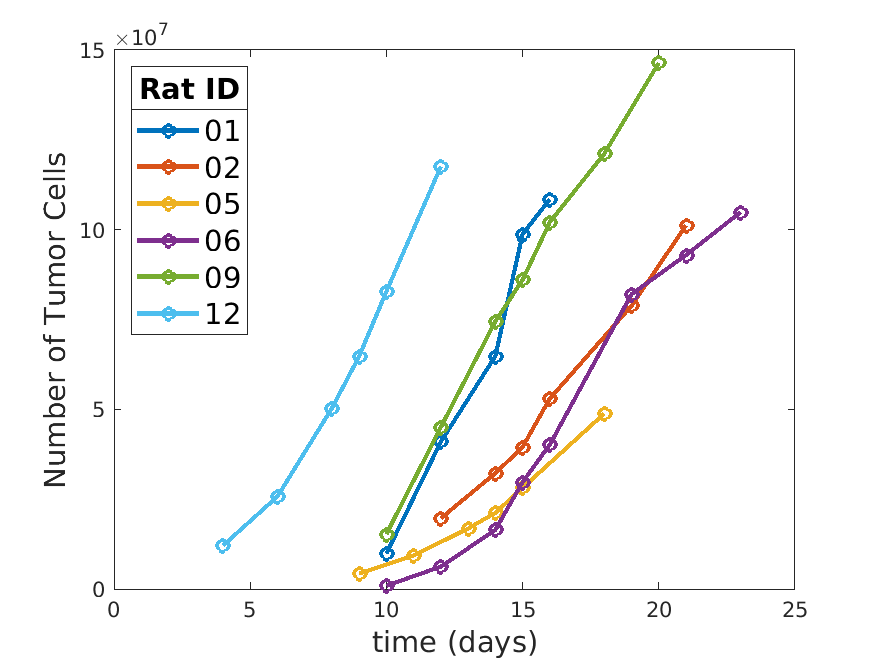
\includegraphics[width=.45\textwidth]{../../mouse-data/images/numtumorcells.png}    	
    	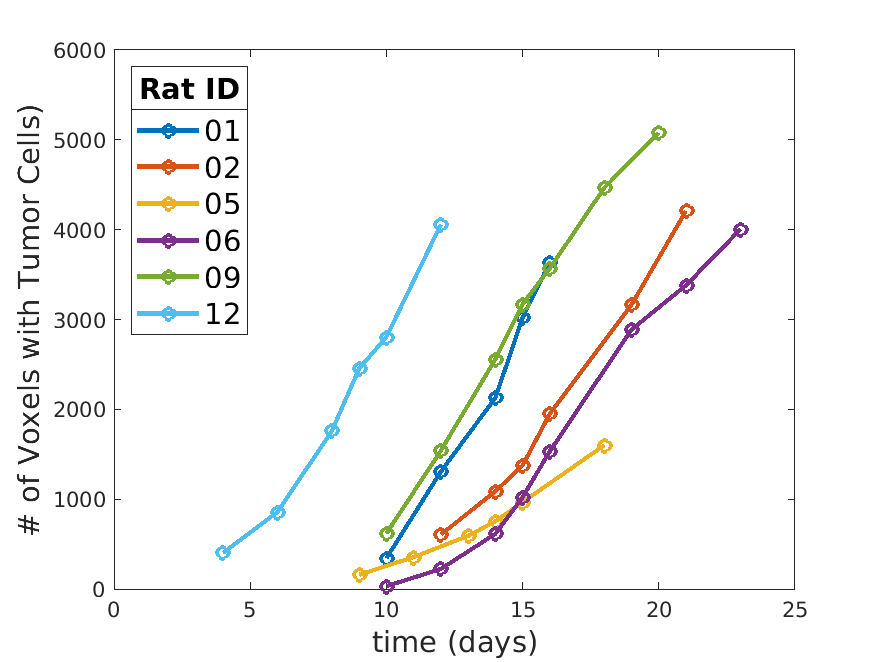
\includegraphics[width=.45\textwidth]{../../mouse-data/images/voxtumorcells.png}
    	\caption{Tumor growth over time in different rats. \textbf{Left:} Cellularity (total measured number of tumor cells). \textbf{Right:} Number of voxels (3D) that have a nonzero amount of tumor cells.}
    	\end{figure}
	\end{minipage}
\end{frame}

\begin{frame}{Comparisons of Tumor Growth Between Rats}
	\begin{minipage}[T][.7\textheight][t]{\textwidth}
		\begin{figure}
    	\centering
    	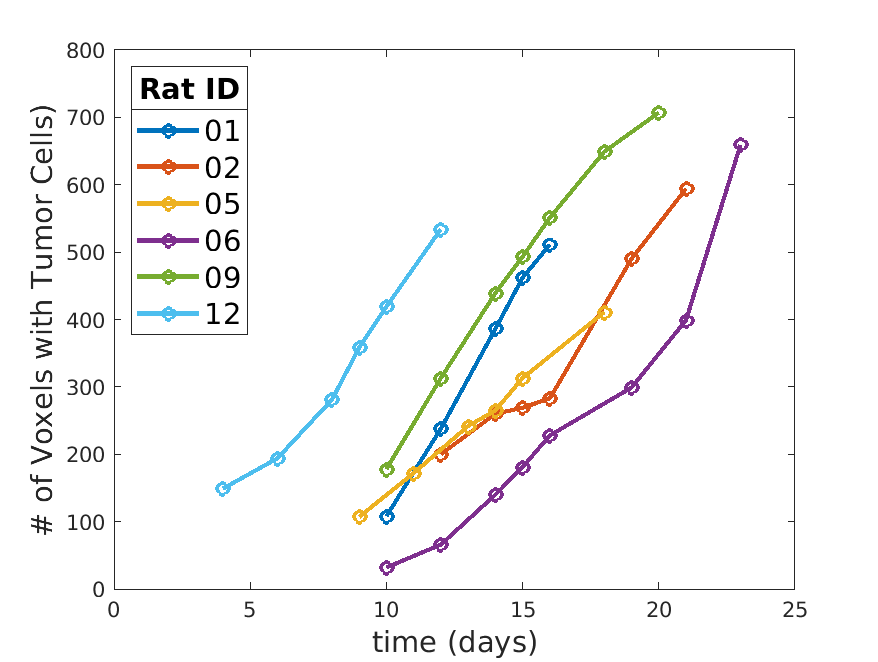
\includegraphics[width=.45\textwidth]{../../mouse-data/images/areatumorcells.png}    	
    	\caption{Number of pixels (2D) with tumor cells in the slice that had the most initial tumor cells for each rat.}
    	\end{figure}
	\end{minipage}
\end{frame}

%===============================================================================
% SLIDE 
\subsection{Individual Rat Data}
%===============================================================================
\begin{frame}{Rat 01, Slice with Max Initial Cellularity}
    \begin{minipage}[t][.7\textheight][t]{\textwidth}
    	\begin{figure}
    	\centering
    	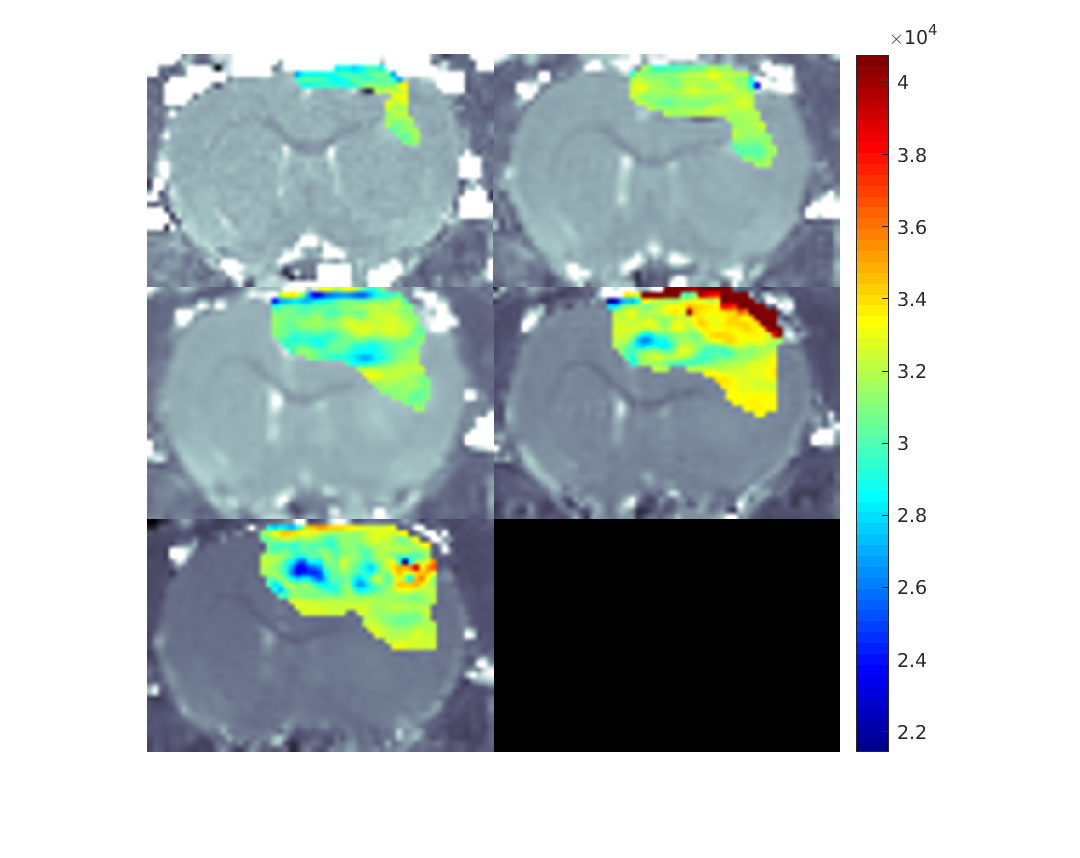
\includegraphics[width=.9\textwidth]{../../mouse-data/images/Montage01.png}
    	\end{figure}
	\end{minipage}  
\end{frame}

\begin{frame}{Rat 02}
    \begin{minipage}[t][.7\textheight][t]{\textwidth}
    	\begin{figure}
    	\centering
    	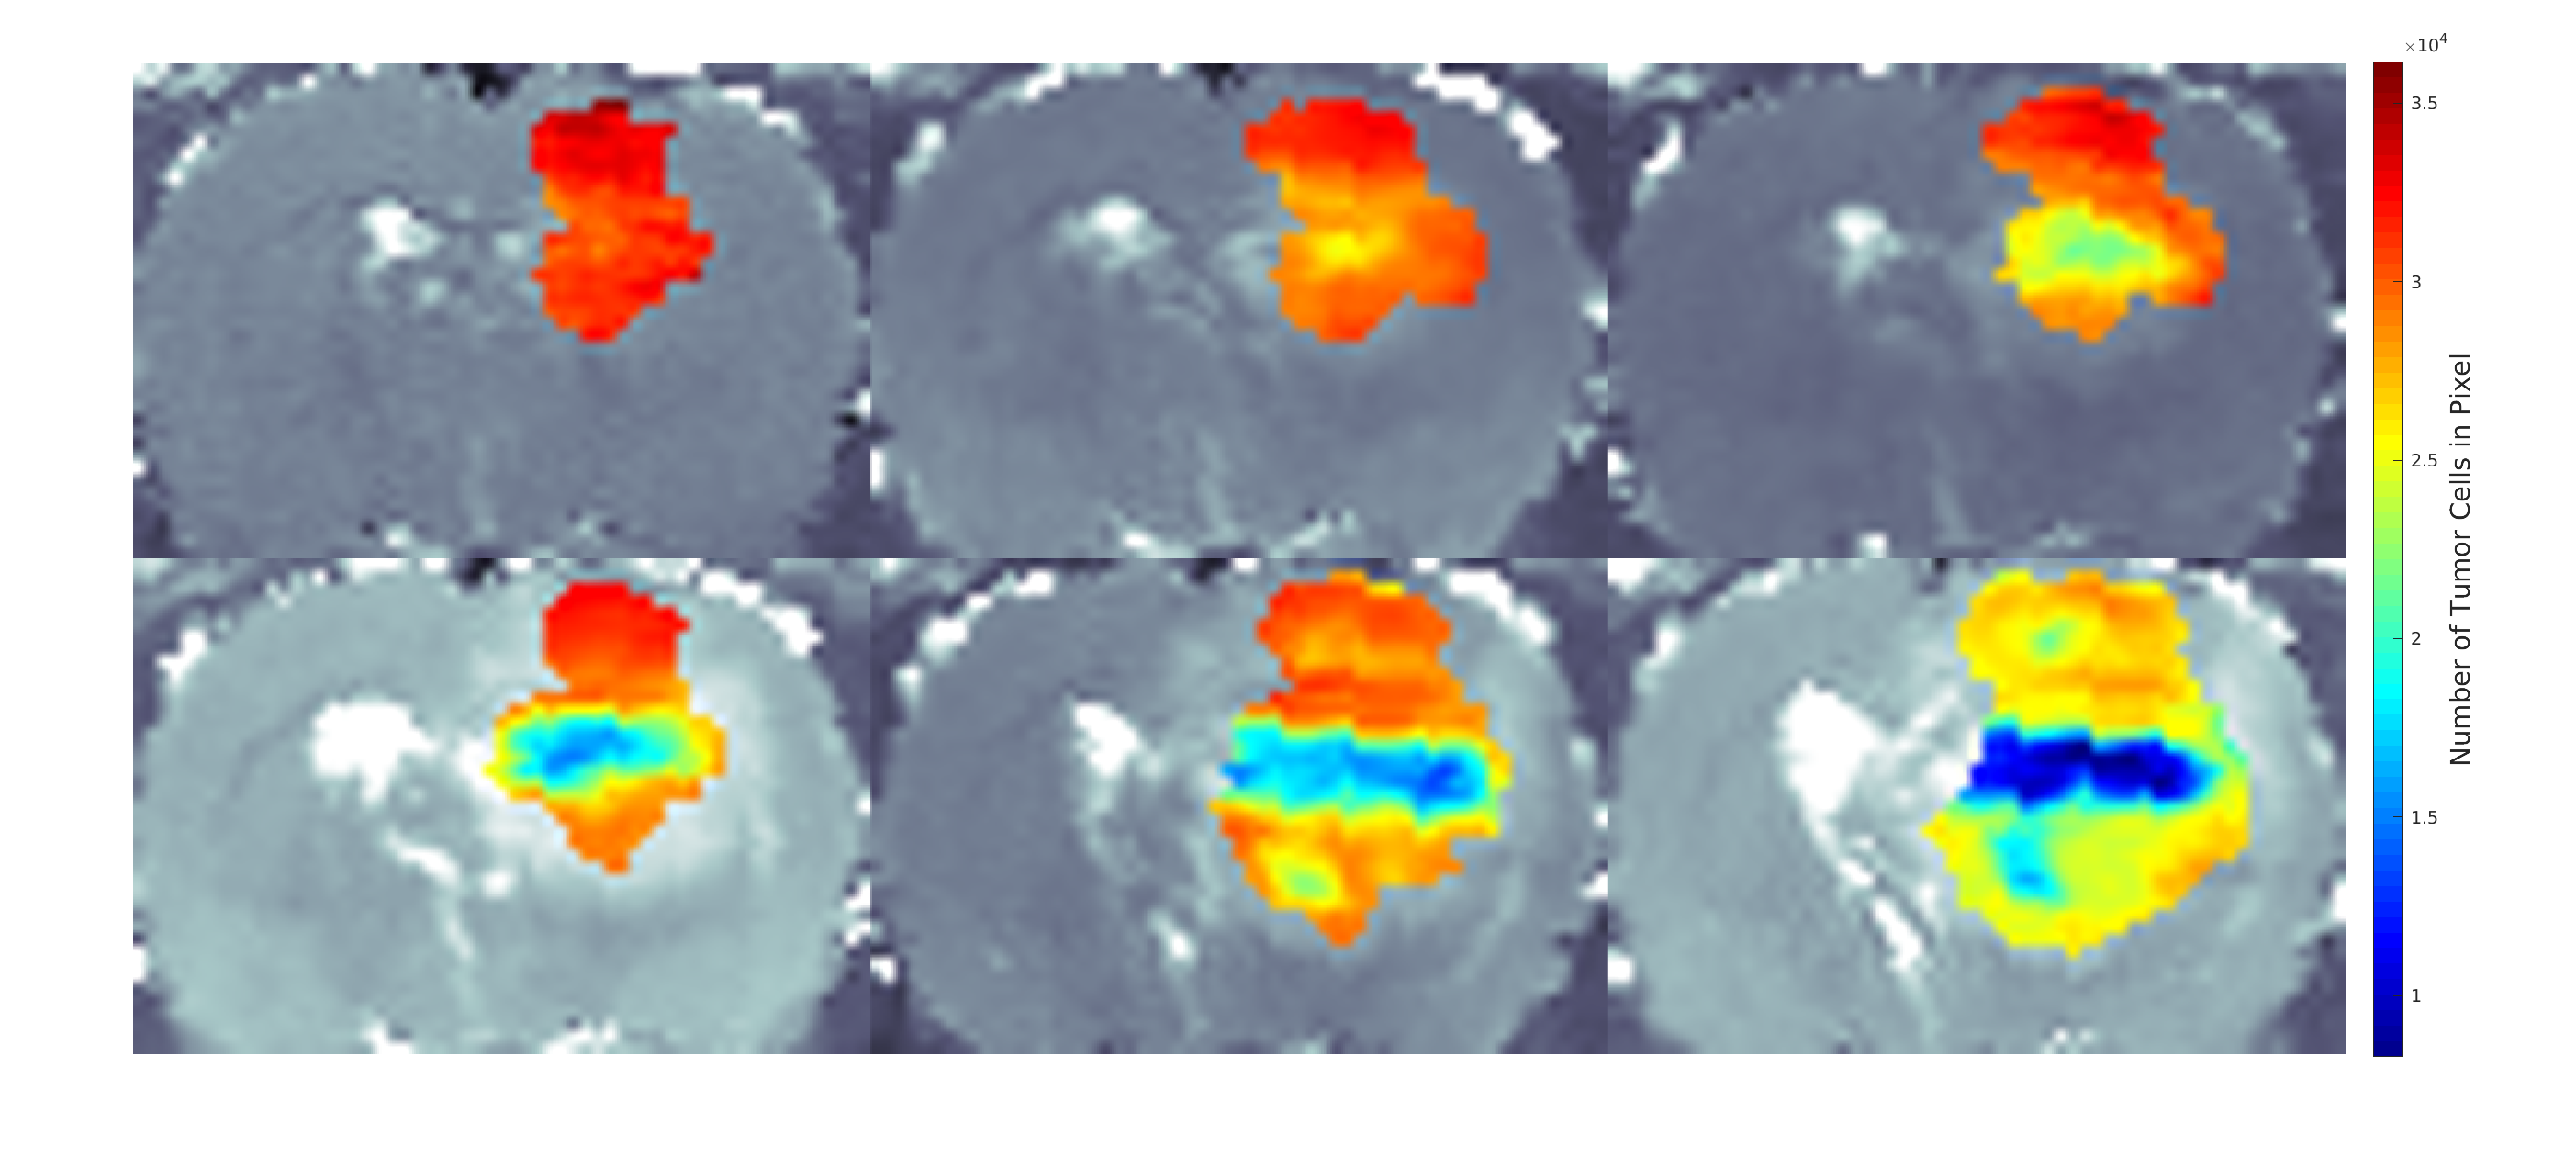
\includegraphics[width=.9\textwidth]{../../mouse-data/images/Montage02.png}
    	\end{figure}
	\end{minipage}  
\end{frame}

\begin{frame}{Rat 05}
    \begin{minipage}[t][.7\textheight][t]{\textwidth}
    	\begin{figure}
    	\centering
    	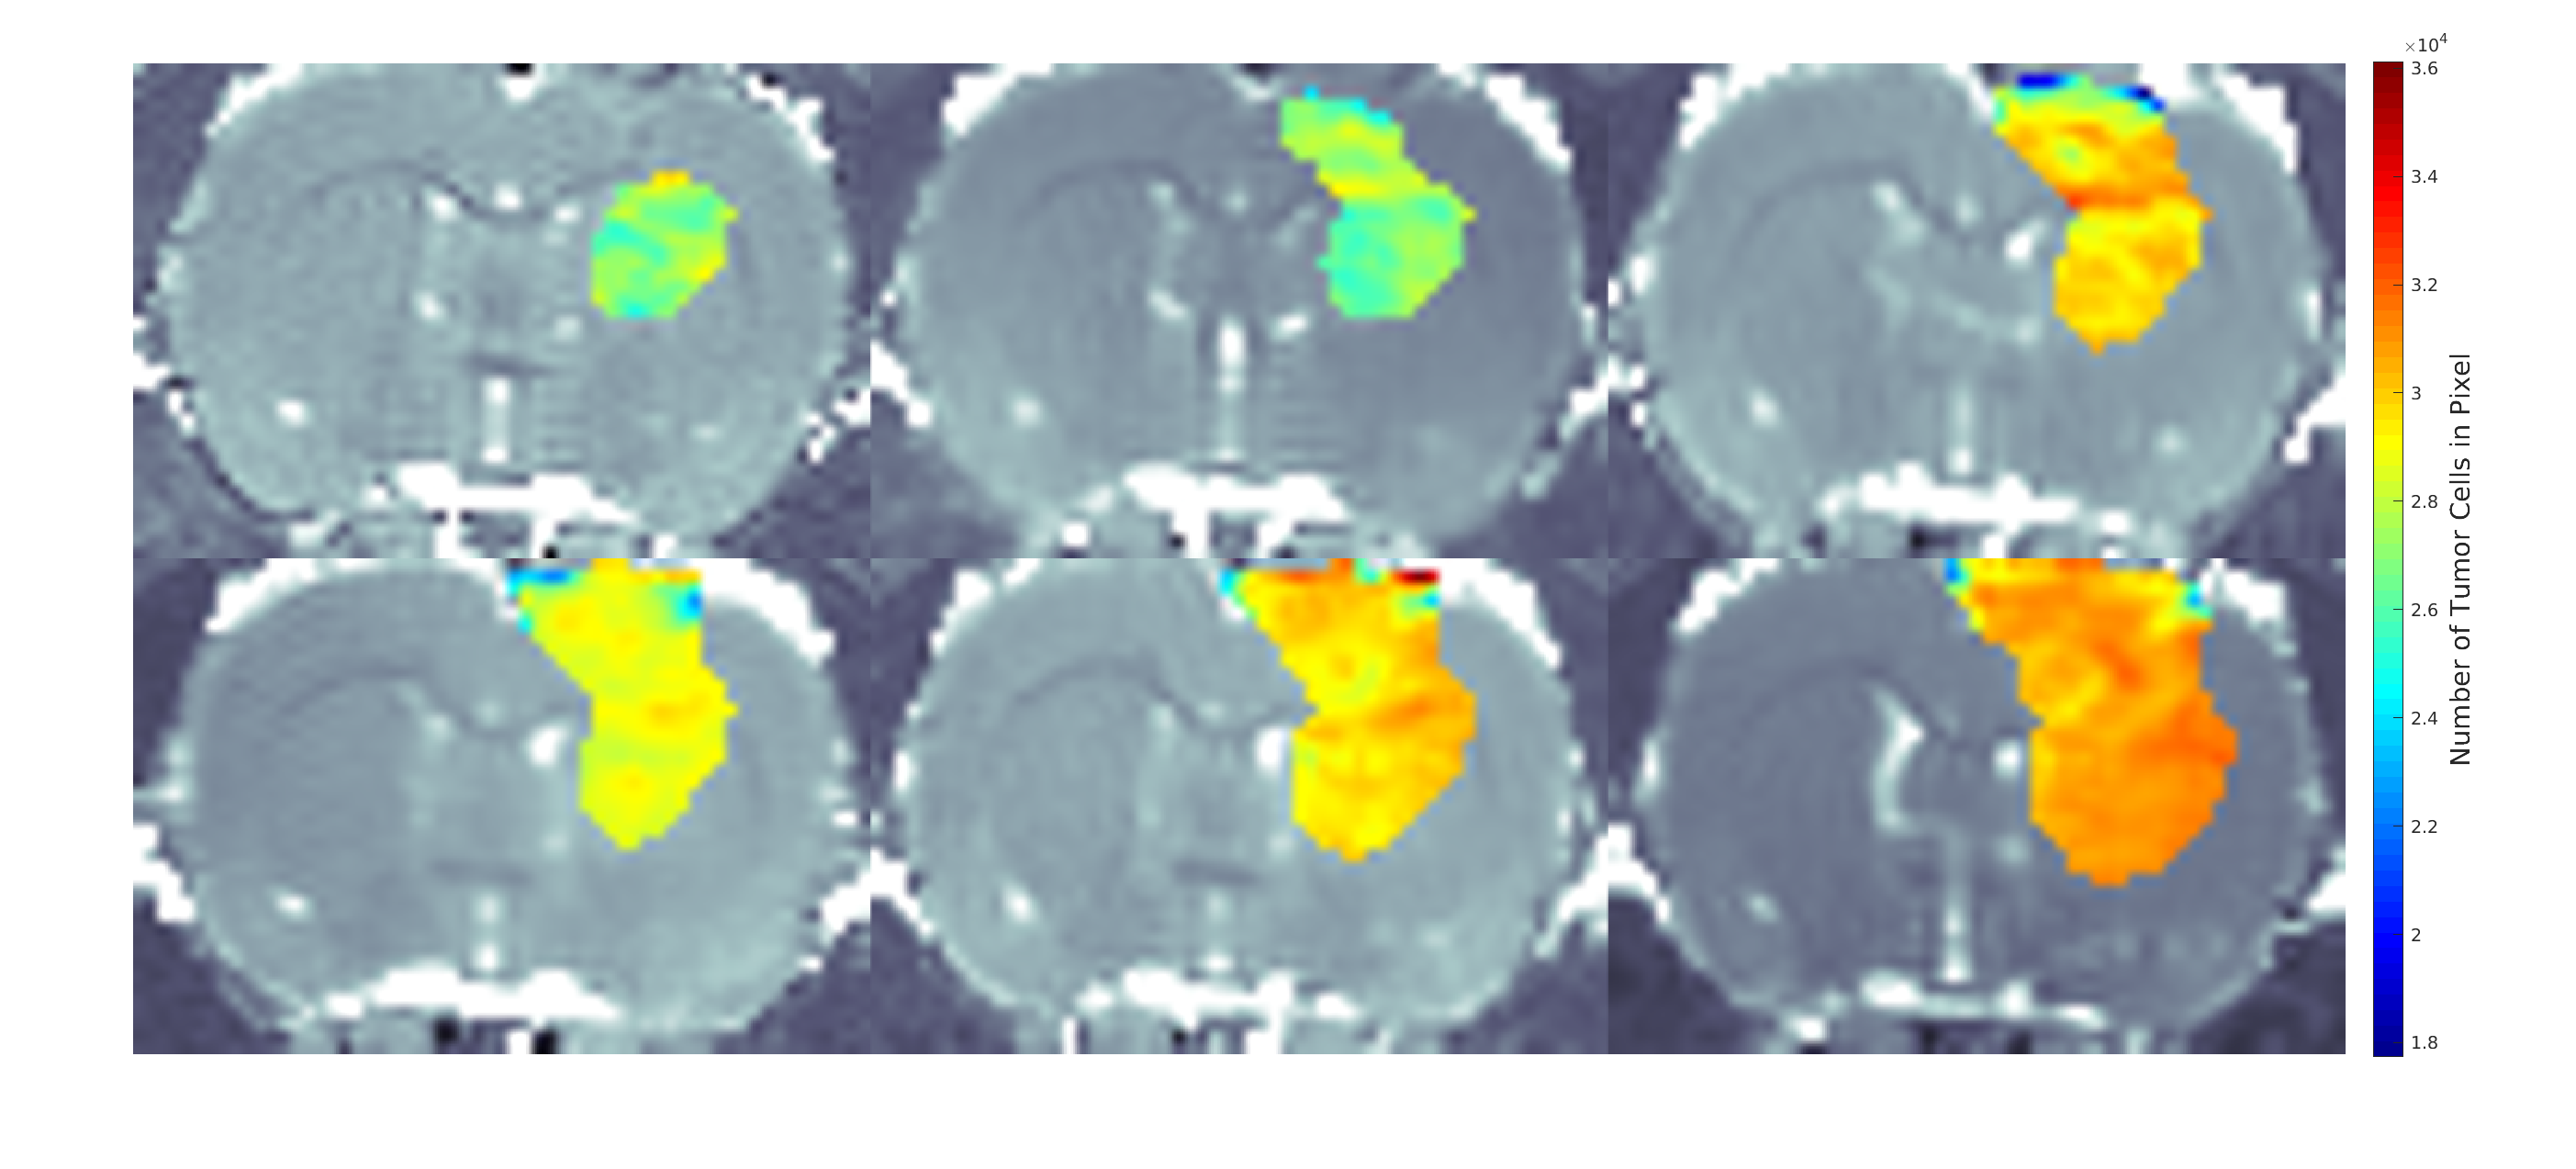
\includegraphics[width=.9\textwidth]{../../mouse-data/images/Montage05.png}
    	\end{figure}
	\end{minipage}  
\end{frame}

\begin{frame}{Rat 06}
    \begin{minipage}[t][.7\textheight][t]{\textwidth}
    	\begin{figure}
    	\centering
    	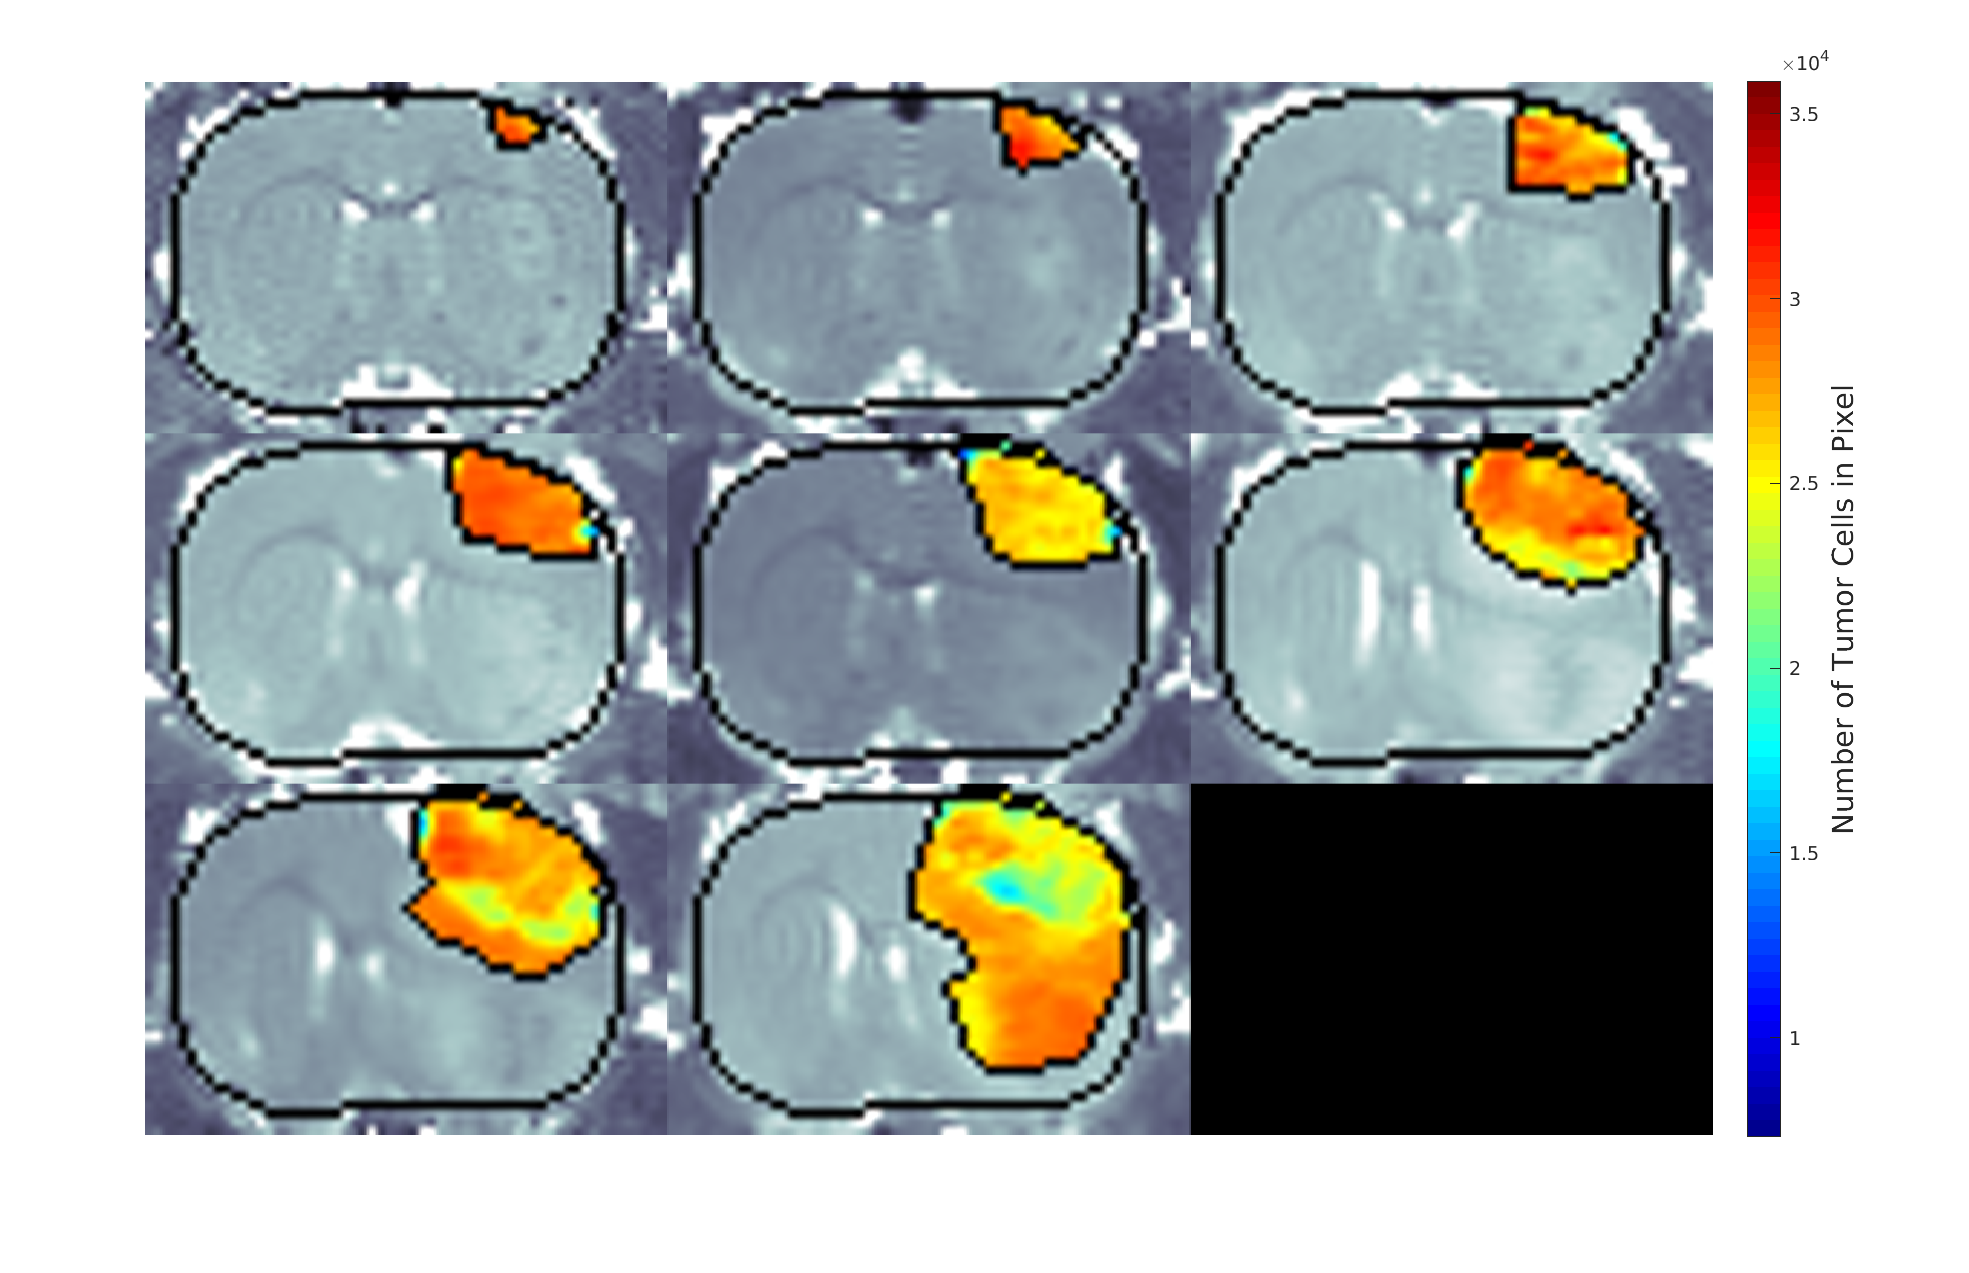
\includegraphics[width=.9\textwidth]{../../mouse-data/images/Montage06.png}
    	\end{figure}
	\end{minipage}  
\end{frame}

\begin{frame}{Rat 09}
    \begin{minipage}[t][.7\textheight][t]{\textwidth}
    	\begin{figure}
    	\centering
    	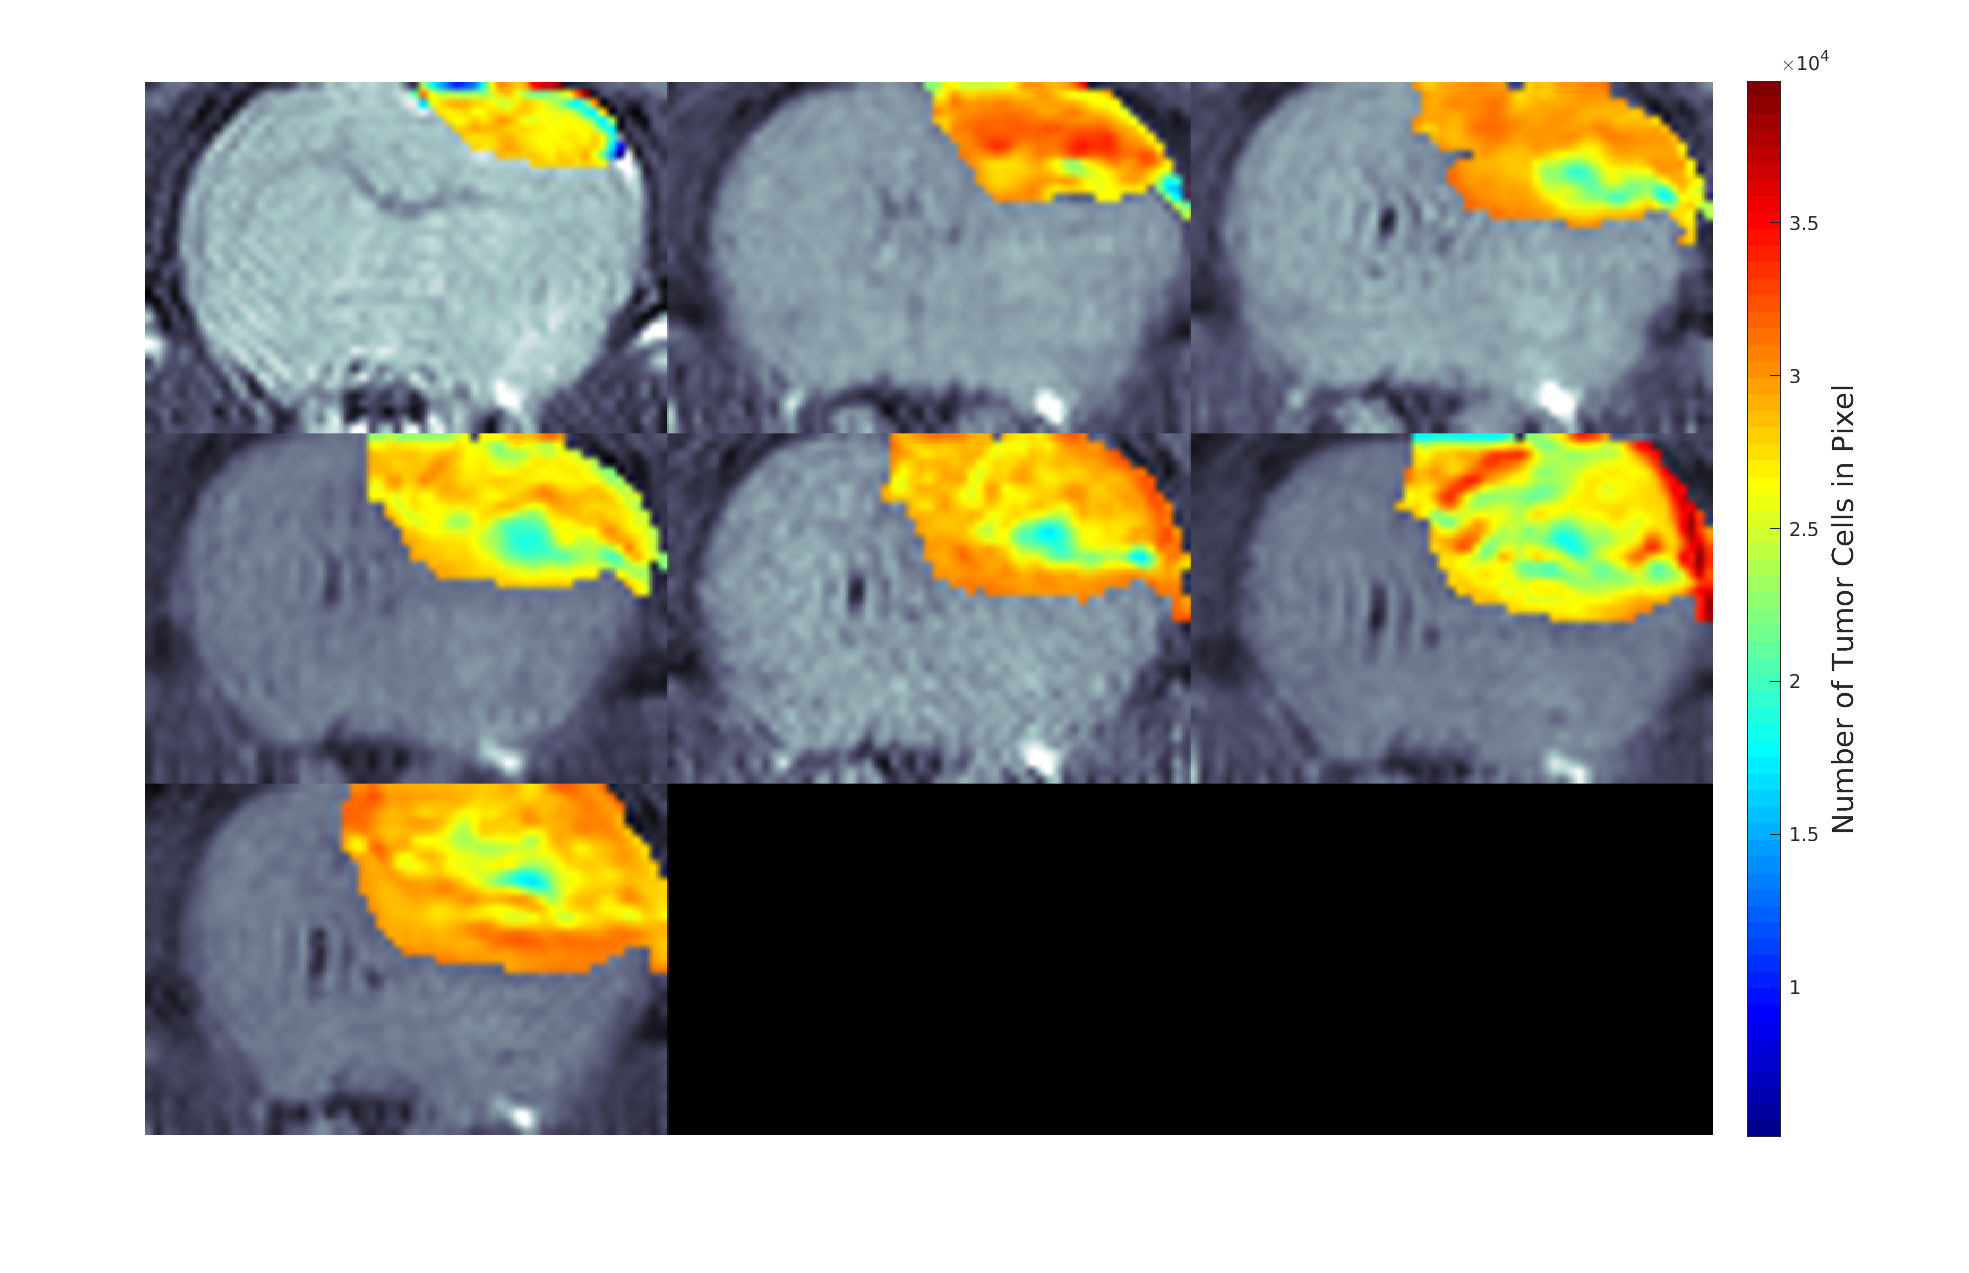
\includegraphics[width=.9\textwidth]{../../mouse-data/images/Montage09.png}
    	\end{figure}
	\end{minipage}  
\end{frame}

\begin{frame}{Rat 12}
    \begin{minipage}[t][.7\textheight][t]{\textwidth}
    	\begin{figure}
    	\centering
    	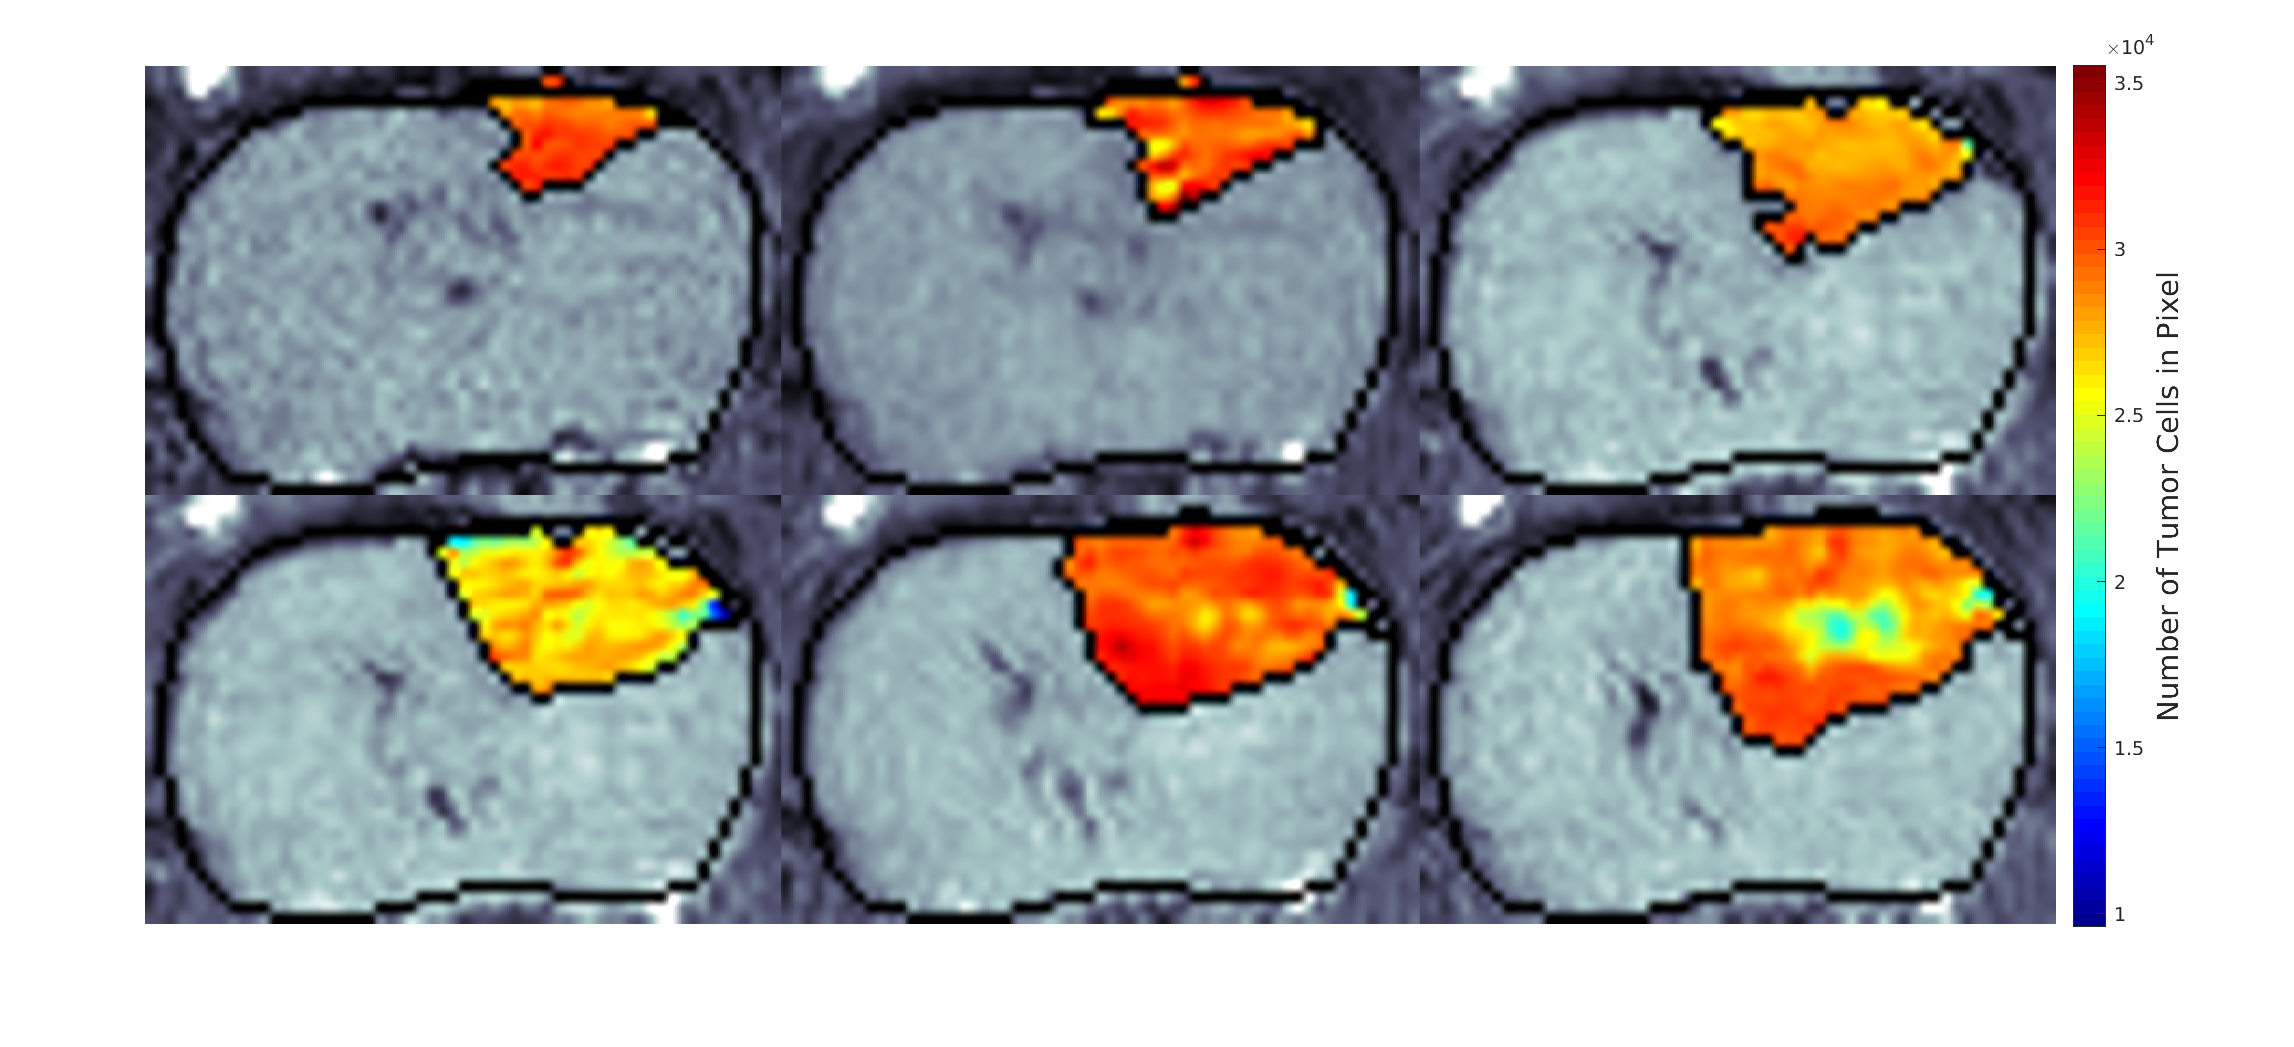
\includegraphics[width=.9\textwidth]{../../mouse-data/images/Montage12.png}
    	\end{figure}
	\end{minipage}  
\end{frame}

\begin{frame}{Meshing}
    \begin{minipage}[t][.7\textheight][t]{\textwidth}
    An example of meshing for rat 05
    	\begin{figure}
    	\centering
    	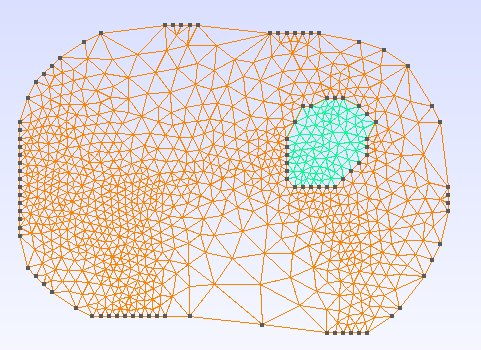
\includegraphics[width=.7\textwidth]{../../mouse-data/images/mesh05.png}
    	\end{figure}
	\end{minipage}  
\end{frame}




\end{document}
